\documentclass[handout]{astro-bookshelf}
\hypersetup{colorlinks=true,linkcolor=blue,citecolor=black,urlcolor=blue}

\usepackage{wasysym}

\graphicspath{{frontmatter/}{coordinates/figs/}{light-telescopes/figs/}{spectroscopy/figs/}{detection-exoplanets/figs/}{beyond-kepler/figs/}{planetary-atmospheres/figs/}{constants-units/figs/}{math-review/figs/}{statistics/figs/}}

\setcounter{secnumdepth}{1}

\usepackage[units,derivatives,vectors,code,symbols]{starType}
\newcommand*{\rhat}{\ensuremath{\bvec{\hat{r}}}}
\newcommand*{\thetahat}{\ensuremath{\bvec{\hat{\theta}}}}
\newcommand*{\rv}{\ensuremath{\bvec{r}}}
\newcommand*{\xv}{\ensuremath{\bvec{x}}}
\newcommand*{\DDtt}[1]{\frac{\dif^{2} #1}{\dif t^{2}}}

\newcommand*{\Earth}{\oplus}
\newcommand*{\Moon}{\leftmoon}

\newcommand*{\joule}{\unitstyle{J}}
\newcommand*{\watt}{\unitstyle{W}}

\newcommand*{\RA}{\ensuremath{\mathrm{RA}}}
\newcommand*{\dec}[3]{%
	\ifthenelse{\isempty{#3}}%
		{\ensuremath{#1^{\circ}\,#2'}}
		{\ensuremath{#1^{\circ}\,#2'\,#3''}}}
\newcommand*{\hrangle}[3]{%
	\ifthenelse{\isempty{#3}}%
		{\ensuremath{#1^{\mathrm{h}}\,#2^{\mathrm{m}}}}
		{\ensuremath{#1^{\mathrm{h}}\,#2^{\mathrm{m}}\,#3^{\mathrm{s}}}}}

\newcommand*{\prob}{\ensuremath{\mathcal{P}}}
\newcommand*{\mean}[1]{\ensuremath{\left\langle#1\right\rangle}}
\newcommand*{\binom}[3]{\ensuremath{\prob_{#1}(#2;#3)}}
\newcommand*{\expect}{\ensuremath{\mathcal{E}}}

\newcommand*{\wt}{\omega t}
\newcommand*{\wot}{\omega_{0} t}
\newcommand*{\wmt}{\omega_{m} t}
\newcommand*{\womw}{(\omega_{0}^{2}-\omega^{2})}
\newcommand*{\gw}{(\Gamma/m)^{2}\omega^{2}}

\newcommand{\newterm}[1]{\textsc{#1}}

\author{Edward Brown}
\publisher{Open Astrophysics Bookshelf}
\date{9 May 2018}


\title{Beyond Kepler's Laws}

\begin{document}

\maketitle

%!TEX root = ../planets-notes.tex

When we studied the two-body problem, we treated the masses as simple points. In reality, they are complex extended objects.  In this chapter, we'll explore some of the effects that arise when we go beyond the simple problem of two massive point particles orbiting one another. 

\section{Tidal forces}
Because a planet is extended, the gravitational force exerted by another mass on it varies across its diameter. As a warm-up, let's imagine putting four test masses some distance from the Earth and letting them free-fall.  We have a camera that is aligned with the center of mass of these four particles and that free-falls with them.
\begin{marginfigure}
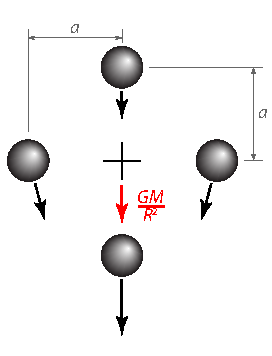
\includegraphics[width=\linewidth]{Tides}
\caption[Four freely falling bodies]{Four freely falling bodies.  In a frame that falls with them, how does their motion appear?
\label{f.tides}}
\end{marginfigure}

Figure~\ref{f.tides} depicts the setup: the particles are a distance $a$ from the center of mass (indicated with a cross) and the center of mass is a distance $R$ from the Earth's center.
When we release the particles and camera, the camera and center of mass both move downward with acceleration $-GM/R^{2}\;\bvec{\hat{z}}$.  Because each particle feels a slightly different gravitational force, however, none of the particles falls with that exact acceleration: the top particle has a lower acceleration and the bottom, higher; while the left and right particles have some horizontal acceleration 
toward the center of mass.

\begin{exercisebox}[Demonstration of tidal acceleration]
\label{ex:simple-tidal}
Compute the difference between the acceleration of each test mass and that of the center of mass.  Expand this difference to lowest order in $a/R$.  This difference is the \newterm{tidal force}.  Sketch the tidal force on each particle from the point of view of the free-falling camera.
\end{exercisebox}

\begin{figure*}[hbtp]
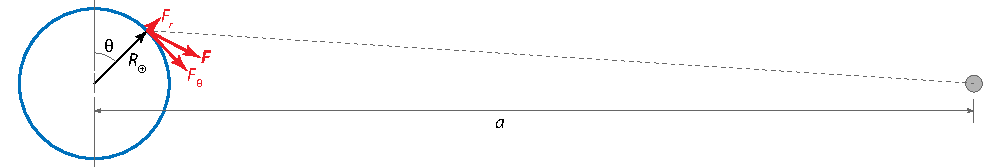
\includegraphics[width=\linewidth]{Earth-Moon-tides}
\caption[Tidal force on the Earth]{Schematic of the tidal force on the Earth raised by the Moon.
\label{f.Earth-Moon-tides}}
\end{figure*}

For the Earth-moon system (Fig.~\ref{f.Earth-Moon-tides}), we can decompose the tidal force exerted by the moon into radial and tangential components.  The Earth-Moon separation is $a = 60.3 R_{\Earth}$, so expanding our expression for the tidal force to lowest order in $R_{\Earth}/a$ is a good approximation.

Upon expanding the tidal acceleration components to lowest order in $R_{\Earth}/a$, the components\sidenote[][2\baselineskip]{The geometry can be worked out by consulting Fig.~\ref{f.Earth-Moon-tides}; it is straightforward, but tedious, and I won't go through the algebra here.} are found to be
\begin{eqnarray}
\label{e.moon-tide-radial}\rhat: &\qquad& \frac{GM_{\Moon}R_{\Earth}}{a^{3}}\left(3\sin^{2}\theta - 1\right)\\
\label{e.moon-tide-tangential}\thetahat: &\qquad& \frac{3GM_{\Moon}R_{\Earth}}{2a^{3}}\sin2\theta.
\end{eqnarray}
\begin{exercisebox}[Radial component of tidal force]
Sanity check: does the radial component of the tidal force, eq.~(\ref{e.moon-tide-radial}), agree with the calculation in Exercise~\ref{ex:simple-tidal}?
\end{exercisebox}
\begin{marginfigure}[5\baselineskip]
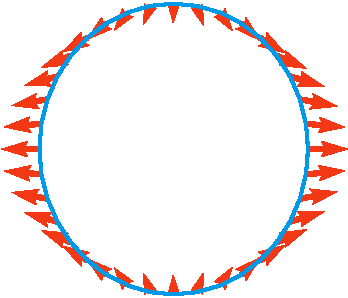
\includegraphics[width=\linewidth]{lunar-tidal-force}
\caption[Components of the tidal force]{Tidal force field exerted by the Moon on the Earth.
\label{f.lunar-tidal-force}}
\end{marginfigure}
\noindent The ratio of the radial component of the tidal acceleration, neglecting the angular dependence, to the Earth's surface gravity is
\[ \frac{M_{\Moon}}{M_{\Earth}}\left(\frac{R_{\Earth}}{a}\right)^{3} = \sci{5.6}{-8}. \]
This is quite small, and you might wonder how the tidal force can produce such large daily flows of water in the ocean.  But consider the tangential component, eq.~(\ref{e.moon-tide-tangential}): it has a maximum at $\theta = 45^{\circ},\,135^{\circ}$ and, although it is also small, there is nothing to oppose it.

\newthought{The Earth's rotational period is shorter than the Moon's orbital period.} Because of viscosity (resistance to flow) the tidal bulge is carried ahead of the line joining the centers of the Earth and Moon (Figure~\ref{f.tidal-torque}).  As a result, the Moon's pull exerts a torque on the Earth and gradually slows its rotation; the oblate Earth in turn exerts a torque on the Moon and gradually forces it to greater orbital separation.

\begin{figure*}
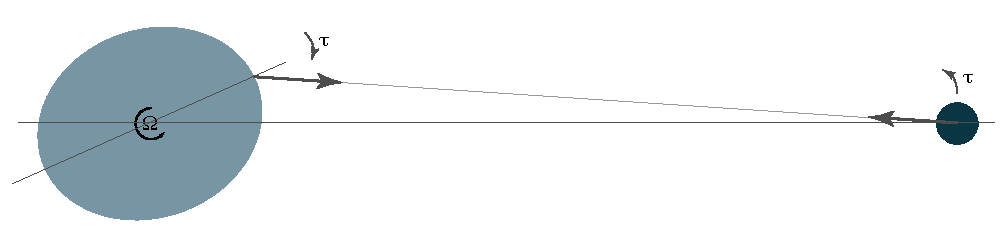
\includegraphics[width=\linewidth]{tidal-torque}
\caption[Torque on the Earth's tidal bulge]{The torque resulting from the misalignment of Earth's tidal bulge.
\label{f.tidal-torque}}
\end{figure*}

\section{Motion in a rotating frame}

To work out the equations of motion in a rotating frame, we start from an inertial frame in polar coordinates.  In this system, the particle is located at $(r,\theta)$; the position vector of the particle is $\rv = r\rhat$. After an internal $\Delta t$, the particle's position is $(r+\Delta r,\theta+\Delta\theta)$, as shown in Fig.~\ref{f.polar-coordinates}.  

\begin{marginfigure}[\baselineskip]
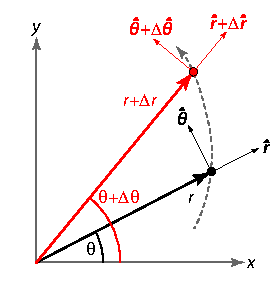
\includegraphics[width=\linewidth]{polar-coordinates}
\caption[Polar coordinates]{Polar coordinates for a particle.
\label{f.polar-coordinates}}
\end{marginfigure}

As the particle moves, both $\rhat$ and $\thetahat$ change as well.  Since both $\rhat$ and $\thetahat$ are unit vectors, only their direction changes with their magnitude remaining constant. Neither vector changes under purely radial motion, $\Delta\theta = 0$.  Under a change in angle $\Delta\theta$, however, both $\rhat$ and $\thetahat$ rotate by an angle $\Delta\theta$, as shown in Fig.~\ref{f.change-polar-unit-vectors}. In the limit $\Delta\theta \to 0$, 
\[ \Delta \rhat \to \Delta\theta \thetahat; \quad \Delta\thetahat \to -\Delta\theta\rhat. \]
Dividing by $\Delta t$ and calling $\omega = \dif\theta/\dif t$ the angular velocity, we have
$\dif\rhat/\dif t = \omega\thetahat$ and $\dif\thetahat/\dif t = -\omega\rhat$.

\begin{marginfigure}[4\baselineskip]
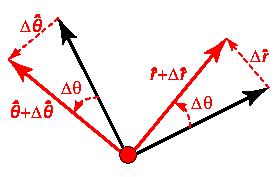
\includegraphics[width=\linewidth]{change-polar-unit-vectors}
\caption[Change in unit vectors under rotation]{Change in the unit vectors $\rhat$ and $\thetahat$ under a change in the angular coordinate $\Delta\theta$.
\label{f.change-polar-unit-vectors}}
\end{marginfigure}

We can then differentiate the particle's position with respect to time to get its velocity in polar coordinates, and then differentiate again to get the acceleration.
\begin{eqnarray}
\DDt{\rv} &=& \DDt{r}\rhat + r\omega\thetahat; \\
\DDtt{\rv} &=& \DDtt{r}\rhat + 2\DDt{r}\omega\thetahat + r \DDt{\omega}\thetahat - r\omega^{2}\rhat.
\label{e.accel-polar}
\end{eqnarray}
Now suppose further that the angular velocity has two parts: $\omega = \Omega+\omega'$, a uniform rotation at velocity $\Omega$ plus a remaining portion $\omega'$.  Further, since $\Omega$ represents uniform rotation, $\dif\Omega/\dif t = 0$ and the acceleration is
\begin{eqnarray}
\frac{1}{m}\bvec{F} = \DDtt{\rv} &=& \left(\DDtt{r} - r\omega'^{2}\right)\rhat + \left(2\DDt{r}\omega' + r\DDt{\omega'}\right)\thetahat\nonumber\\
 && -r\Omega^{2}\rhat + 2\Omega\left(\DDt{r}\thetahat - r\omega'\rhat\right).
\label{e.full-accel}
\end{eqnarray}
Here $\bvec{F}$ is the force in an inertial frame.

Now the first two terms on the right-hand side are just the acceleration $\dif^{2}\rv'/\dif t^{2}$ that an observer rotating with velocity $\Omega$ would write down (cf.\ eq.~[\ref{e.accel-polar}]).  Hence, if we move the last two terms of equation (\ref{e.full-accel}) to the left, we are left with the equations of motion in a rotating frame,
\marginnote{We also make the identification \[ v_{r} = \dif r/\dif t,\quad v_{\theta} = r\omega'.\]}
\begin{equation}\label{e.motion-rotating}
\DDtt{\rv'} = \frac{1}{m}\bvec{F}_{\mathrm{rot}} = \frac{1}{m}\bvec{F} 
	+  \underbrace{r\Omega^{2}\rhat}_{\textrm{centrifugal}}
	+	\underbrace{2\Omega\left(v_{\theta}\rhat - v_{r}\thetahat \right)}_{\textrm{Coriolis}}.
\end{equation}
The \newterm{centrifugal} force is outwards (along \rhat); the \newterm{Coriolis} force depends on velocity and deflects the motion of a particle at right angles to its velocity\sidenote{That is, if you are moving in the \rhat\ direction, the Coriolis force is in the \thetahat\ direction, and vice versa.}.  If you've ever tried to walk in a straight line on a spinning merry-go-round, then you've met the Coriolis force.

\begin{exercisebox}[Coriolis acceleration on merry-go-round]
\label{ex:coriolis}
Figure~\ref{f.coriolis-exercise} depicts a merry-go-round rotating counter-clockwise with velocity $\Omega > 0$.  Four points, A--D are moving as shown.  Draw the deflections of their trajectories due to the Coriolis force.
\end{exercisebox}
\begin{marginfigure}[4\baselineskip]
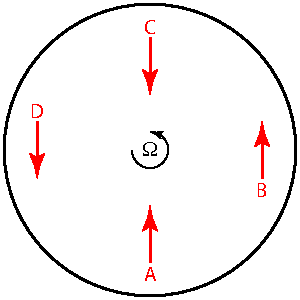
\includegraphics[width=\linewidth]{coriolis-exercise}
\caption[Movement on a merry-go-round]{Schematic for Exercise~\ref{ex:coriolis}.
\label{f.coriolis-exercise}}
\end{marginfigure}

\section{Lagrange and Roche}
For analyzing the motion of a test particle in the vicinity of two massive orbiting bodies, we transform to a frame with an origin at the center of mass.  The bodies have masses $M_{1}$ and $M_{2}$, and we take $M_{1}$ to be the more massive of the two. The bodies are located at coordinates
\begin{eqnarray}
	M_{1}:&\qquad& x_{1} = -a\frac{M_{2}}{M},\,y_{1} = 0;\\
	M_{2}:&\qquad& x_{2} = a\frac{M_{1}}{M},\,y_{2} = 0,
\end{eqnarray}
Here $M = M_{1}+M_{2}$ is the total mass of the two bodies and $a$ their separation. Our coordinate system rotates with angular velocity $\Omega = GM/a^{3}$.

Let's check that our rotating coordinate system is consistent: since $M_{2}$ is at rest, the net force on it vanishes, so from equation~(\ref{e.motion-rotating}),
\[ -\frac{GM_{1}}{a^{2}} + a\frac{M_{1}}{M_{1}+M_{2}}\Omega^{2} = 0, \]
or
\[ P_{\mathrm{orb}}^{2} = \left(\frac{2\pi}{\Omega}\right)^{2} = \frac{4\pi^{2}}{GM}a^{3}. \]
This is just what we would expect from Kepler's law.

Now we are in a position to ask, are there any points where a particle could sit at rest in this frame?\marginnote{Remember, ``at rest in this frame'' means the particle is co-rotating with our two masses.}
Between the two masses, for example, we expect that the net force must vanish at some point. The acceleration of a test mass located at $\bvec{r}$ is 
\begin{equation}\label{e.test-mass-acceleration-x}
\DDtt{\rv} = -\frac{GM_{1}}{|\rv-\rv_{1}|^{3}}(\rv-\rv_{1}) - \frac{GM_{2}}{|\rv-\rv_{2}|^{3}}(\rv-\rv_{2}) + \frac{G(M_{1}+M_{2})}{a^{3}} \rv.
\end{equation}
Along the $x$-axis, points where a particle would feel no acceleration are given by the roots of the equations
\begin{eqnarray*}
	x < x_{1}:&\qquad& \frac{GM_{1}}{(x_{1}-x)^{2}} + \frac{GM_{2}}{(x_{2}-x)^{2}} + \frac{G(M_{1}+M_{2})}{a^{3}} x = 0;\\
	x_{1} < x < x_{2}:&\qquad& -\frac{GM_{1}}{(x-x_{1})^{2}} + \frac{GM_{2}}{(x_{2}-x)^{2}} + \frac{G(M_{1}+M_{2})}{a^{3}} x = 0;\\
	x_{2} < x:&\qquad& \frac{GM_{1}}{(x-x_{1})^{2}} + \frac{GM_{2}}{(x-x_{2})^{2}} + \frac{G(M_{1}+M_{2})}{a^{3}} x = 0.
\end{eqnarray*}
This is a nasty quintic equation; if, however, we take the limit $M_{2}\ll M_{1}$ then after some inspired algebra we find that there are three roots, which are the first three \newterm{Lagrange points}:
\begin{eqnarray*}
L_{1} &\qquad& x_{L1} \approx a\left\{\frac{M_{1}}{M_{1}+M_{2}} - \left[\frac{M_{2}}{3(M_{1}+M_{2})}\right]^{1/3}\right\};\\
L_{2} &\qquad& x_{L2} \approx a\left\{\frac{M_{1}}{M_{1}+M_{2}} + \left[\frac{M_{2}}{3(M_{1}+M_{2})}\right]^{1/3}\right\};\\
L_{3} &\qquad& x_{L3} \approx a\left\{-\frac{M_{1}+2M_{2}}{M_{1}+M_{2}} + \frac{7M_{2}}{12M_{1}}\right\}.
\end{eqnarray*}
These points are depicted in Fig.~\ref{f.Roche} for a system with $M_{2} = 0.05\,M_{1}$.
The remaining two Lagrange points $L_{4}$ and $L_{5}$ form equilateral triangles with $M_{1}$ and $M_{2}$.
\begin{marginfigure}[-8\baselineskip]
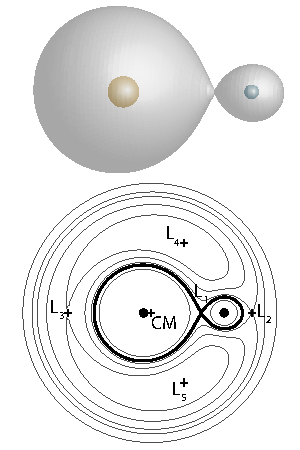
\includegraphics[width=\linewidth]{Roche}
\caption{Lagrange points for a system with $M_{2} = 0.1\,M_{1}$.
\label{f.Roche}}
\end{marginfigure}
We can draw an equipotential surface (in the rotating frame) that crosses through $L_{1}$: the surface is dumbbell-shaped and forms two \newterm{Roche lobes} (Fig.~\ref{f.Roche}) that touch at $L_{1}$.  Within each lobe the gradient of the potential is inward toward the center of the lobe.

\begin{exercisebox}[Vanishing acceleration at $L_{4}$]
Show that the acceleration vanishes at $L_{4}$:
\begin{enumerate}\renewcommand{\labelenumi}{\alph{enumi})}
   \item Find the coordinates of $L_{4}$;
   \item Compute the net gravitational acceleration, due to both $M_{1}$ and $M_{2}$, on a particle at point $L_{4}$ and show that it points toward the center of mass; then
   \item Show that the gravitational acceleration cancels the centrifugal, so that the net acceleration vanishes.
\end{enumerate}
\end{exercisebox}

\newthought{From the expressions for $L_{1}$ and $L_{2}$, we notice that} they can be written
as
\sidenote{Recall that
\[ a\frac{M_{1}}{M_{1}+M_{2}} = x_{2}, \]
the location of body 2.}
\[ 
	x_{L1} \approx x_{2} - R_{\mathrm{H}};\quad x_{L2}\approx x_{2} + R_{\mathrm{H}},
\]
with
\[ R_{\mathrm{H}}\approx a\left[\frac{M_{2}}{3(M_{1}+M_{2})}\right]^{1/3}. \]
Particles within a sphere of radius $R_{\mathrm{H}}$ are dominated by the gravitational attraction of $M_{2}$; $R_{\mathrm{H}}$ is called the \newterm{Hill radius}.

\begin{exercisebox}[Hill radius of the Sun-Jupiter system]
Compute the Hill radius for the Sun-Jupiter system.
\end{exercisebox}

\begin{exercisebox}[Overflow of Roche lobe]
Speculate on what would happen if $M_{2}$ had an atmosphere that extended outside its Roche lobe.
\end{exercisebox}

\section{Angular Momentum}\label{s.angular-momentum}
There is another way of looking at the spin-orbit interaction of the Earth and Moon.  What is the spin angular momentum of the Earth? What is the orbital angular momentum of the Moon and Earth? How do they compare?

The angular momentum of a particle of mass $m$ is
\begin{equation}\label{e.def-L}
	\bvec{L} = \bvec{r}\vcross m\bvec{v}.
\end{equation}
For a particle in a circular orbit, $\bvec{v} = r\Omega \thetahat$; using Kepler's law, we have
\[	L = mr^{2}\Omega = m\left(GMr\right)^{1/2}, \]
where $r$ is the distance from the center of mass.  The direction of $\bvec{L}$ is perpendicular to the plane of the orbit.  For two bodies orbiting a common center of mass, the problem is equivalent to a single particle of mass
\[ \mu = \frac{M_{1}M_{2}}{M_{1}+M_{2}} \]
orbiting a \emph{fixed} mass $M_{1}+M_{2}$ at a distance $a$, where $a$ is the separation of the two bodies.  Hence the orbital angular momentum of the two-body system is
\begin{equation}\label{orbital-2-two-body}
	L = \mu a^{2}\Omega = \frac{M_{1}M_{2}}{M_{1}+M_{2}}\left[G\left(M_{1}+M_{2}\right)a\right]^{1/2}.
\end{equation}
The orbital angular momentum increases with separation $a$.

Now for the spin angular momentum. Let's take a simple case, that of a sphere of uniform density $\rho = 3M/(4\pi R^{3})$. The sphere rotates uniformly with angular velocity $\Omega$. In this case, the spin angular momentum (see Box~\ref{sb.angular-momentum-uniform-sphere}) is
\begin{equation}\label{e.ang-momentum-sphere}
	L = \frac{2}{5} MR^{2}\Omega.
\end{equation}
If the density is not uniform, but is higher toward the center, then the angular momentum is reduced. For example, the Earth's moment of inertia is\cite{Lissauer2013Fundamental-Pla} $I_{\Earth} = 0.331 M_{\Earth}R_{\Earth}^{2}$.

\begin{exercisebox}[Orbital angular momentum of the Earth-Moon system]
Compute the orbital angular momentum of the Earth-Moon system.  Compute the spin angular momentum of the Earth. Compare the two.
\end{exercisebox}

\begin{exercisebox}[Effect of central concentration on the moment of inertia]
Explain why having a higher density toward the center of a planet would reduce its moment of inertia.
\end{exercisebox}

\begin{sidebar}[Angular momentum of a uniform sphere]
\label{sb.angular-momentum-uniform-sphere}
To find the total angular momentum, we add up the contributions from infinitesimal bits.  To make this easy, we'll use the geometry shown below.  We'll divide our sphere into shells, each a distance $r$ from the center and of thickness $\dif r$.  Then we'll slice each shell into rings of width $r\,\dif\theta$.  We'll add up the angular momentum of the rings to find the angular momentum of shell, and then sum up the angular momentum of the shells to get the total.
\begin{center}
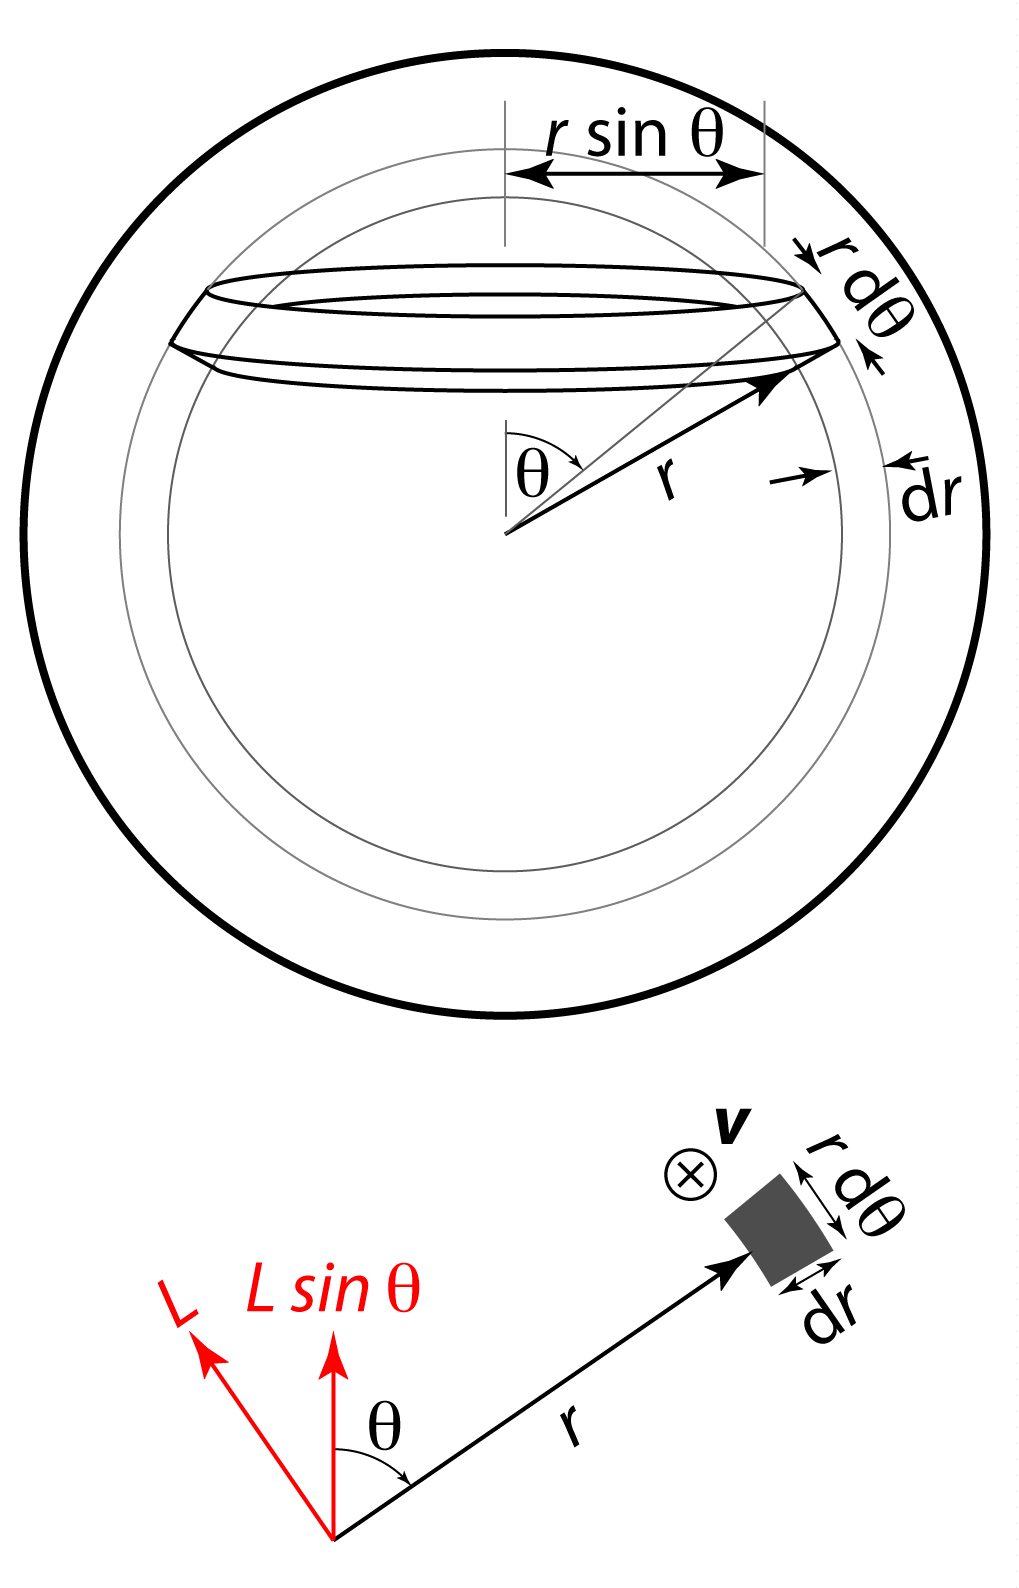
\includegraphics[width=0.5\linewidth]{Inertia}
\end{center}

Consider a cross-section of a ring.  The angular momentum is perpendicular to both $\bvec{r}$ and $\bvec{v}$; when we add up all of the pieces around the ring, the horizontal parts cancel, leaving the vertical part.  The mass of the ring is $\rho\times 2\pi r\sin\theta\,\dif r\,r\dif\theta$; the velocity is $r\sin\theta \times \Omega$.  The vertical component of the ring's angular momentum is therefore
\[
	\dif L_{\mathrm{ring}} = 2\pi \rho\Omega r^{4}\sin^{3}\theta\, \dif \theta \,\dif r.
\]
To get the angular momentum of a shell, we integrate over $\theta$:
\[
	\dif L_{\mathrm{shell}} = 2\pi\rho\Omega r^{4}\,\dif r\,\int_{0}^{\pi}\sin^{3}\theta\,\dif\theta.
\]
To do the integral, write $\sin^{3}\theta = (1-\cos^{2}\theta)\sin\theta$; then change variables to $\mu = \cos \theta$: in that case $\dif\mu = -\sin^\theta\,\dif\theta$, $\mu(\theta = 0) = 1$, and $\mu(\theta=\pi)=-1$.  The integral is then
\[
	\int_{0}^{\pi}\sin^{3}\theta\,\dif\theta = \int_{-1}^{1}(1-\mu^{2})\,\dif\mu 
		= \frac{4}{3},
\]
and the angular momentum of our shell is
\[
	\dif L_{\mathrm{shell}} = \frac{8\pi}{3}\rho\Omega r^{4}\,\dif r.
\]
Finally, integrate over $r$ to get the angular momentum of the sphere,
\begin{equation}
	L = \frac{8\pi}{3}\rho\Omega \int_{0}^{R}r^{4}\,\dif r = \frac{8\pi}{15}\rho\Omega R^{5} = \frac{2}{5} MR^{2}\Omega.
\end{equation}
In this last equation we substituted for $\rho = 3M/(4\pi R^{3})$. 
\end{sidebar}

\section{Orbital resonances in the solar system}
Planets, moons, and other minor bodies in solar system have made millions to billions of orbits. 
Suppose an asteroid had an orbital period that was one-half that of Jupiter's---that is, the asteroid made two orbits for every one orbit of Jupiter. At the point of closest approach, Jupiter exerts a small gravitational tug on the asteroid. Since the orbital periods are in a 2:1 ratio, these tugs always happen at the same point in the asteroid's orbit and will eventually perturb the orbital motion, just as pumping your legs in phase with the period of a swing will cause it's amplitude to increase. Even a small perturbing force, if applied near a natural frequency of a system, can eventually produce a large response when applied over such a long dynamical time. 

There are many bodies in the solar system that are locked into a stable resonance. For example, Pluto is locked into a stable 2:3 resonance with Neptune (that is, Pluto completes 2 orbits for every 3 of Neptune), and the Jovian moons Io, Europa, and Ganymede are locked into a 1:2:4 resonance. Resonances can also lead to instability, in which a body's orbit is distorted to the point that it crosses the orbit of another planet, at which point that body either collides with the other planet or is scattered out of the solar system.  For example, the Kirkwood gap in the asteroid belt is located at the 3:1 resonance with Jupiter (see Fig.~2.10 of \citetalt{Lissauer2013Fundamental-Pla}). Numerical calculations find that the precession of Mercury's perihelion is coming into resonance with that of Jupiter, leading to a 1\% chance over the next \val{5}{\Giga\yr} of Mercury colliding with the Sun or Venus, and a smaller possibility of the entire inner solar system becoming unstable\cite{Laskar2009Existence-of-co} over that time.

\newthought{Torques exerted on a planet's equatorial bulge} by other solar system bodies can cause that planet's obliquity to vary.  Saturn's large (relative to Jupiter) axial tilt is thought to be caused by a spin-orbit resonance between the precession of Saturn's axis the precession of Neptune's orbital plane\cite{Ward2004Tilting-Saturn.}.  Mars's axial tilt wanders considerably over a few Myr timescale and has reached tilts as large as $60^{\circ}$ in the past.  The large moment of inertia of the Earth-Moon system keeps Earth's axial tilt from wandering to such extreme values; nevertheless, the Earth's inclination does oscillate by $<1^{\circ}$ on a $\val{40\,000}{\yr}$ timescale.  This wandering of the inclination, along with variations in the orbital eccentricity, are thought to explain the quasi-periodic ice ages on Earth over the last few million years\cite{Zachos2001Trends-Rhythms-}.





\bibliographystyle{plainnat}
\bibliography{bibs/AST208}

\end{document}
